\setlength{\footskip}{8mm}

\chapter{Introduction}

\textit{Some text.}

\section{Overview}

Human monitoring is therefore becoming
increasingly expensive and ineffective as the torrent of video data
increases. For instance, in a CCTV monitoring room (see
Figure \ref{fig:monitoring}), security operators are required to
monitor 24 hours a day and be ready to take action when an alarm
occurs. 

\begin{figure}[t]
  \centering
  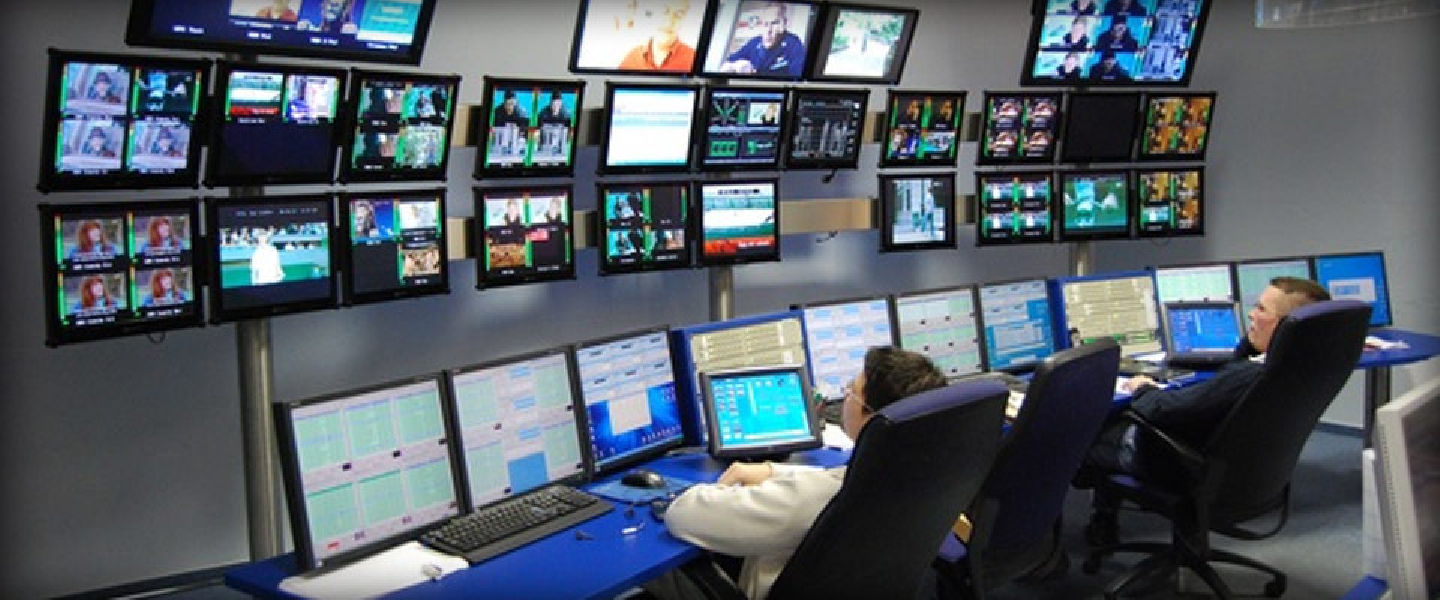
\includegraphics[width=5in]{figures/monitoring}
  \caption[CCTV monitoring room.]{\small CCTV monitoring
    room. Reprinted from the Twenty First Security Web site
    (\url{http://www.twentyfirstsecurity.com.au/}).}
  \label{fig:monitoring}
\end{figure}

\section{Problem Statement}

Some text ...

\section{Objectives}

Some text ...

\section{Limitations and Scope}

Some text ...

\section{Thesis Outline}

I organize the rest of this dissertation as follows.

In Chapter \ref{ch:literature-review}, I describe the literature review.

In Chapter \ref{ch:methodology}, I propose my methodology.

In Chapter \ref{ch:results}, I present the experimental results.

Finally, in Chapter \ref{ch:conclusion}, I conclude my thesis.

\FloatBarrier
